% !TEX program = pdflatex
% =====================================================================
%  Plantilla de memoria TFG / TFM
%  Grau en Enginyeria Informàtica · Escola Politècnica Superior · UdL
%
%  1. Rellena config/datos.tex (autor, título, director, idioma, citas).
%  2. Pon la portada oficial de la EPS en portada/portada.pdf.
%  3. Escribe cada capítulo en capitulos/ y cada apéndice en apendices/.
%  4. Para depositar: cambia mode=review por mode=final (más abajo)
%     y comprueba que compila SIN errores ni avisos de referencias.
%  Lee guia/guia_tfg.pdf antes de empezar.
% =====================================================================
\documentclass[12pt,a4paper,oneside,openany]{book}

% =====================================================================
%  DATOS DEL TRABAJO  ·  rellena SOLO este fichero para personalizar
%  la memoria, los informes de seguimiento y la portada provisional.
% =====================================================================

% --- Tipo de trabajo (tal como aparece en la portada oficial, en catalán)
\newcommand{\tfgtipo}{Treball de Fi de Grau}       % o: Treball de Fi de Màster
\newcommand{\tfgsigla}{TFG}                        % o: TFM

% --- Estudiante y título (el título debe ser IDÉNTICO al de la propuesta
%     administrativa y al de la portada oficial)
\newcommand{\tfgautor}{Nombre Apellido1 Apellido2}
\newcommand{\tfgtitulo}{Título del trabajo: subtítulo que diga qué se ha hecho}

% --- Titulación y centro (en la lengua de la portada oficial: catalán)
\newcommand{\tfgtitulacion}{Grau en Enginyeria Informàtica}
\newcommand{\tfgcentro}{Escola Politècnica Superior}
\newcommand{\tfgcampus}{Campus d'Igualada}         % o: Campus de Cappont (Lleida)
\newcommand{\tfguniversidad}{Universitat de Lleida}

% --- Dirección. Deja \tfgcodirector vacío ({}) si no hay codirector/a.
\newcommand{\tfgdirector}{Nombre y apellidos del director/a}
\newcommand{\tfgcodirector}{}

% --- Presentación (mes en catalán, como en la portada oficial: Juny, Juliol, Setembre)
\newcommand{\tfgmes}{Juliol}
\newcommand{\tfganyo}{2027}
\newcommand{\tfgcurso}{2026--2027}

% --- Palabras clave (3-6), en los tres idiomas del resumen
\newcommand{\tfgclavesES}{palabra clave 1, palabra clave 2, palabra clave 3}
\newcommand{\tfgclavesCA}{paraula clau 1, paraula clau 2, paraula clau 3}
\newcommand{\tfgclavesEN}{keyword 1, keyword 2, keyword 3}

% --- Idioma principal del documento: spanish | catalan | english
%     (cambia "Capítulo", "Índice", "Figura", "Tabla"... automáticamente)
\newcommand{\idiomadocumento}{spanish}

% --- Estilo de citas: ieee (numérico [1], recomendado) | apa (autor-año)
%     Elige UNO y no lo mezcles nunca.
\newcommand{\estilocitas}{ieee}

% --- Enlaces que aparecen en el Apéndice A (repositorio y vídeo demo)
\newcommand{\tfgrepo}{https://github.com/usuario/repositorio}
\newcommand{\tfgversion}{v1.0.0}                   % tag o commit entregado
\newcommand{\tfgvideo}{https://youtu.be/XXXXXXXXXXX}

% =====================================================================
%  PREÁMBULO COMÚN (memoria, informes y guía)
%  Normalmente NO hace falta tocar este fichero: los datos van en
%  config/datos.tex. Si añades paquetes, hazlo al final, en la zona
%  marcada, y comprueba que el documento sigue compilando sin errores.
%  Requiere: \idiomadocumento y \estilocitas (definidos en datos.tex).
% =====================================================================

% --- Codificación, fuentes y microtipografía --------------------------
\usepackage[T1]{fontenc}
\usepackage[utf8]{inputenc}
\usepackage{lmodern}
\usepackage[babel=true]{microtype}

% --- Idiomas: castellano, catalán e inglés; el principal sale de datos.tex
%     es-tabla        -> «Tabla» en vez de «Cuadro»
%     es-noshorthands -> evita conflictos de < > " con TikZ y tablas
%     es-nodecimaldot -> 3.5 en fórmulas no se convierte en 3,5
\edef\tfgbabelopts{english,catalan,spanish,main=\idiomadocumento}
\expandafter\usepackage\expandafter[\tfgbabelopts,es-tabla,es-noshorthands,es-nodecimaldot]{babel}
\usepackage{csquotes}

% --- Página: A4, márgenes, interlineado 1,15, párrafos sin línea en blanco
\usepackage[a4paper,top=2.5cm,bottom=2.5cm,left=3cm,right=2.5cm,headheight=15pt]{geometry}
\usepackage{setspace}
\setstretch{1.15}
\usepackage[skip=6pt plus 2pt]{parskip}   % separación entre párrafos sin dobles saltos
\raggedbottom
% Sin líneas viudas ni huérfanas
\clubpenalty=10000
\widowpenalty=10000
\displaywidowpenalty=10000

% --- Colores, figuras, tablas y diagramas -----------------------------
\usepackage[table,dvipsnames]{xcolor}
\usepackage{graphicx}
\graphicspath{{figuras/}}
\usepackage{float}
\usepackage[section]{placeins}            % las figuras no "huyen" a otra sección
\usepackage{booktabs,tabularx,multirow,array,longtable}
\newcolumntype{L}{>{\raggedright\arraybackslash}X}
\newcolumntype{C}{>{\centering\arraybackslash}X}
\renewcommand{\arraystretch}{1.2}
\usepackage{amsmath,amssymb}
\usepackage{siunitx}                      % \qty{100}{ms}, \num{12345}: cifras y unidades
\usepackage{tikz}
\usetikzlibrary{arrows.meta,positioning,fit,backgrounds,shapes.geometric,babel}
\usepackage{pgfgantt}
\usepackage{qrcode}
\usepackage{enumitem}
\setlist{itemsep=2pt,topsep=4pt}

% --- Pies de figura y tabla: centrados, breves; tablas con el pie ARRIBA
\usepackage[font=small,labelfont=bf,labelsep=colon,justification=centering,
            singlelinecheck=true]{caption}
\captionsetup[table]{position=top,skip=6pt}
\captionsetup[figure]{skip=6pt}
\usepackage[list=true]{subcaption}

% \fuente{...}: línea de fuente bajo la figura o la tabla (OBLIGATORIA).
%   \fuente{Elaboración propia.}   \fuente{Adaptado de \cite{clave}.}
\newcommand{\fuente}[1]{\par\vspace{3pt}{\centering\footnotesize\fuentename: #1\par}}

% --- Código fuente --------------------------------------------------
\usepackage{listings}
\lstset{
  basicstyle=\ttfamily\small, columns=fullflexible, keepspaces=true,
  breaklines=true, breakatwhitespace=false, tabsize=2,
  frame=tb, framesep=4pt, numbers=left, numberstyle=\tiny\color{gray}, numbersep=6pt,
  keywordstyle=\color{RoyalBlue}\bfseries, commentstyle=\color{ForestGreen}\itshape,
  stringstyle=\color{BrickRed}, showstringspaces=false, captionpos=b,
  floatplacement=htbp,  % con [float] en cada listado, el código no se parte entre páginas
  extendedchars=true,
  literate={á}{{\'a}}1 {é}{{\'e}}1 {í}{{\'i}}1 {ó}{{\'o}}1 {ú}{{\'u}}1
           {Á}{{\'A}}1 {É}{{\'E}}1 {Í}{{\'I}}1 {Ó}{{\'O}}1 {Ú}{{\'U}}1
           {à}{{\`a}}1 {è}{{\`e}}1 {ò}{{\`o}}1 {ï}{{\"i}}1 {ü}{{\"u}}1
           {ñ}{{\~n}}1 {Ñ}{{\~N}}1 {ç}{{\c c}}1 {Ç}{{\c C}}1 {·}{{$\cdot$}}1
           {¿}{{?`}}1 {¡}{{!`}}1
}

% --- Acrónimos: \ac{TFG} -> 1.ª vez «Trabajo de Fin de Grado (TFG)», después «TFG»
\usepackage[printonlyused]{acronym}

% --- Bibliografía (biblatex + biber). Un ÚNICO estilo en todo el documento.
\edef\tfgbibopts{backend=biber,style=\estilocitas}
\expandafter\usepackage\expandafter[\tfgbibopts]{biblatex}
\usepackage{xurl}                          % URLs largas que se parten bien
% Fecha de consulta y URL en el idioma del documento (nunca «Accessed» en un
% texto en castellano):  «Consultado el 15 de nov. de 2026. Disponible en: URL»
\DefineBibliographyStrings{spanish}{urlseen={Consultado el}, url={Disponible en}}
\DefineBibliographyStrings{catalan}{urlseen={Consultat el}, url={Disponible a}}

% --- Textos que dependen del idioma --------------------------------------
\addto\captionsspanish{%
  \def\fuentename{Fuente}\def\acronimosname{Acrónimos}%
  \def\lstlistingname{Listado}\def\lstlistlistingname{Índice de listados}%
  \def\resumenname{Resumen}\def\clavesname{Palabras clave}%
  \sisetup{output-decimal-marker={,}}}
\addto\captionscatalan{%
  \def\fuentename{Font}\def\acronimosname{Acrònims}%
  \def\lstlistingname{Llistat}\def\lstlistlistingname{Índex de llistats}%
  \def\resumenname{Resum}\def\clavesname{Paraules clau}%
  \sisetup{output-decimal-marker={,}}}
\addto\captionsenglish{%
  \def\fuentename{Source}\def\acronimosname{Acronyms}%
  \def\lstlistingname{Listing}\def\lstlistlistingname{List of Listings}%
  \def\resumenname{Abstract}\def\clavesname{Keywords}%
  \sisetup{output-decimal-marker={.}}}

% --- Encabezados de capítulo y profundidad del índice ----------------
\usepackage{titlesec}
\ifdefined\chapter
  \titleformat{\chapter}[display]
    {\normalfont\bfseries\huge\raggedright\hyphenpenalty=10000}
    {\large\chaptertitlename~\thechapter}{6pt}{\huge}
    [\vspace{2pt}\titlerule]
  \titlespacing*{\chapter}{0pt}{0pt}{20pt}
\fi
% Títulos sin palabras partidas por guiones
\titleformat*{\section}{\normalfont\Large\bfseries\raggedright\hyphenpenalty=10000}
\titleformat*{\subsection}{\normalfont\large\bfseries\raggedright\hyphenpenalty=10000}
\setcounter{secnumdepth}{2}   % numera hasta X.Y.Z; no uses un 4.º nivel
\setcounter{tocdepth}{1}      % el índice muestra capítulos y secciones (máx. 2 niveles)

% --- Cabecera y pie: número de página centrado abajo ----------------
\usepackage{fancyhdr}
\pagestyle{fancy}
\fancyhf{}
\fancyhead[R]{\small\nouppercase{\leftmark}}
\fancyfoot[C]{\thepage}
\renewcommand{\headrulewidth}{0.4pt}
\fancypagestyle{plain}{\fancyhf{}\fancyfoot[C]{\thepage}\renewcommand{\headrulewidth}{0pt}}

% --- Enlaces y metadatos del PDF (hyperref casi al final) --------------
\usepackage[colorlinks=true,linkcolor=black,citecolor=black,
            urlcolor=MidnightBlue,bookmarksnumbered=true,pdfusetitle]{hyperref}
\usepackage{bookmark}

% --- Zona para tus paquetes y comandos propios -----------------------
% \usepackage{...}

\usepackage{pdfpages}

% --- Notas de revisión (revnotes.sty) --------------------------------
%  mode=review : se ven las notas y los \pending (mientras escribes)
%  mode=final  : desaparecen las notas; un \pending olvidado da ERROR,
%                así no se deposita nada con texto provisional.
\usepackage[mode=review]{revnotes}
\revauthor{vitor}{Director}{revTeal}      % \vitornote{...} notas del director
\revauthor{alumno}{Estudiante}{revBlue}   % \alumnonote{...} notas propias

\addbibresource{bibliografia.bib}

\hypersetup{pdftitle={\tfgtitulo},pdfauthor={\tfgautor},
            pdfsubject={\tfgtipo{} - \tfgtitulacion},pdfkeywords={\tfgclavesES}}

\begin{document}

% =====================================================================
%  PARTE PRELIMINAR (numeración romana, no aparece en el índice general)
% =====================================================================
\frontmatter

% Portada oficial EPS si existe; si no, la provisional.
\IfFileExists{portada/portada.pdf}
  {\includepdf[pages=1]{portada/portada.pdf}}
  {% =====================================================================
%  PORTADA PROVISIONAL
%  Solo se usa mientras NO exista portada/portada.pdf.
%  La versión que se deposita DEBE llevar la portada oficial de la EPS
%  (ver portada/README.md). Por eso aquí hay un \pending: en mode=final
%  la compilación falla hasta que pongas la portada oficial.
% =====================================================================
\begin{titlepage}
  \thispagestyle{empty}
  \centering
  {\large\scshape \tfguniversidad\par}
  {\normalsize \tfgcentro{} · \tfgcampus\par}
  \vspace{3cm}
  {\Huge\bfseries\MakeUppercase{\tfgtipo}\par}
  \vspace{2.5cm}
  \begin{flushleft}
    \renewcommand{\arraystretch}{1.6}
    \begin{tabular}{@{}p{0.30\textwidth}p{0.62\textwidth}@{}}
      \textbf{Estudiant:}  & \tfgautor \\
      \textbf{Titulació:}  & \tfgtitulacion \\
      \textbf{Títol:}      & \tfgtitulo \\
      \textbf{Director/a:} & \tfgdirector \\
      \ifx\tfgcodirector\empty\else \textbf{Codirector/a:} & \tfgcodirector \\ \fi
      \textbf{Presentació:} & Mes: \tfgmes \quad Any: \tfganyo \\
    \end{tabular}
  \end{flushleft}
  \vfill
  \fbox{\parbox{0.9\textwidth}{\centering\small
    \pending{Portada provisional: sustituir por la portada oficial de la EPS
    (portada/portada.pdf)}}}
\end{titlepage}
}

% Un resumen por idioma, cada uno en su propia página.
% =====================================================================
%  RESUMEN (castellano) · una página · 200-300 palabras
%  Debe decir, por este orden: problema y contexto (2-3 frases), qué se ha
%  hecho y cómo, qué se ha obtenido (con cifras) y qué aporta.
%  No es una introducción: el lector tiene que saber el RESULTADO.
%  Resum y Abstract dicen lo mismo en su idioma, cada uno en su página.
% =====================================================================
\begin{otherlanguage}{spanish}
\chapter*{\resumenname}
\pdfbookmark[0]{\resumenname}{resumen}

% Ejemplo de estructura (sustitúyelo por tu propio resumen):
Reservar un espacio de estudio en el campus obliga hoy a consultar varias
fuentes y no permite saber si una sala está libre en ese momento. Este trabajo
presenta \emph{SalaLibre}, una aplicación móvil y un servicio web que muestran
la ocupación de las salas en tiempo real y permiten reservarlas en dos pasos.

La solución se ha desarrollado con una metodología iterativa en tres
incrementos. La aplicación Android se comunica con una API REST que guarda las
reservas en una base de datos relacional y notifica los cambios a los clientes.
Se han definido doce requisitos funcionales y cinco no funcionales, y cada uno
se ha validado con, al menos, un caso de prueba.

Las pruebas de carga muestran que, con caché, la latencia media se mantiene por
debajo de \qty{100}{ms} hasta 400 usuarios concurrentes, mientras que la versión
inicial superaba ese umbral a partir de 200. Una prueba de usabilidad con ocho
estudiantes obtuvo una puntuación SUS media de 81 sobre 100. Los datos de este ejemplo son ficticios.

\vspace{1em}
\noindent\textbf{\clavesname:} \tfgclavesES
\end{otherlanguage}
\cleardoublepage
      % castellano
% =====================================================================
%  RESUM (català) · una pàgina · mateix contingut que el Resumen
% =====================================================================
\begin{otherlanguage}{catalan}
\chapter*{\resumenname}
\pdfbookmark[0]{\resumenname}{resum}

% Exemple d'estructura (substitueix-lo pel teu resum):
Reservar un espai d'estudi al campus obliga avui a consultar diverses fonts i
no permet saber si una sala és lliure en aquell moment. Aquest treball presenta
\emph{SalaLibre}, una aplicació mòbil i un servei web que mostren l'ocupació de
les sales en temps real i permeten reservar-les en dos passos.

La solució s'ha desenvolupat amb una metodologia iterativa en tres increments.
L'aplicació Android es comunica amb una API REST que desa les reserves en una
base de dades relacional i notifica els canvis als clients. S'han definit dotze
requisits funcionals i cinc de no funcionals, i cadascun s'ha validat amb, com
a mínim, un cas de prova.

Les proves de càrrega mostren que, amb memòria cau, la latència mitjana es manté
per sota dels \qty{100}{ms} fins a 400 usuaris concurrents, mentre que la versió
inicial superava aquest llindar a partir de 200. Una prova d'usabilitat amb vuit
estudiants va obtenir una puntuació SUS mitjana de 81 sobre 100. Les dades d'aquest exemple són fictícies.

\vspace{1em}
\noindent\textbf{\clavesname:} \tfgclavesCA
\end{otherlanguage}
\cleardoublepage
        % catalán
% =====================================================================
%  ABSTRACT (English) · one page · same content as the Resumen
% =====================================================================
\begin{otherlanguage}{english}
\chapter*{\resumenname}
\pdfbookmark[0]{\resumenname}{abstract}

% Example structure (replace it with your own abstract):
Booking a study room on campus currently requires checking several sources, and
it is not possible to know whether a room is free right now. This work presents
\emph{SalaLibre}, a mobile application and a web service that show room
occupancy in real time and allow a room to be booked in two steps.

The solution was developed with an iterative methodology in three increments.
The Android application communicates with a REST API that stores bookings in a
relational database and notifies clients of every change. Twelve functional and
five non-functional requirements were defined, and each one was validated with
at least one test case.

Load tests show that, with caching, the mean latency stays below \qty{100}{ms} up
to 400 concurrent users, whereas the initial version exceeded that threshold
from 200 users onwards. A usability test with eight students obtained a mean
SUS score of 81 out of 100.
The data in this example are fictitious.

\vspace{1em}
\noindent\textbf{\clavesname:} \tfgclavesEN
\end{otherlanguage}
\cleardoublepage
     % inglés

% =====================================================================
%  AGRADECIMIENTOS (opcional) · breve, media página como máximo
% =====================================================================
\chapter*{Agradecimientos}
\pdfbookmark[0]{Agradecimientos}{agradecimientos}

Escribe aquí, si quieres, unas líneas de agradecimiento a las personas e
instituciones que han hecho posible este trabajo. Si el trabajo se ha hecho
dentro de un grupo de investigación, un proyecto o una empresa, indícalo aquí
con su nombre oficial.

\cleardoublepage

% =====================================================================
%  DECLARACIÓN DE USO DE HERRAMIENTAS DE INTELIGENCIA ARTIFICIAL
%  OBLIGATORIA si has usado cualquier herramienta de IA generativa
%  (asistentes de chat, autocompletado de código, traducción, generación
%  de imágenes...). Si no has usado ninguna, dilo en una frase.
%  Sé concreto: herramienta, para qué, en qué partes y cómo lo revisaste.
%  Lo que NO se acepta como aportación propia: el análisis, la discusión
%  de resultados ni las conclusiones generadas por IA.
% =====================================================================
\chapter*{Declaración de uso de herramientas de IA}
\pdfbookmark[0]{Declaración de uso de IA}{declaracionia}

Durante la elaboración de este trabajo se han utilizado las herramientas de
inteligencia artificial generativa que se indican a continuación. Tras su uso,
el autor o la autora ha revisado y editado todo el contenido afectado y asume la
plena responsabilidad del contenido de esta memoria y del código entregado.

% Tabla sin número ni pie: no debe aparecer en el índice de tablas.
\begin{center}
  \small
  \begin{tabularx}{\textwidth}{@{}>{\raggedright\arraybackslash}p{2.6cm}LL>{\raggedright\arraybackslash}p{3.2cm}@{}}
    \toprule
    \textbf{Herramienta} & \textbf{Uso concreto} & \textbf{Partes afectadas} & \textbf{Revisión} \\
    \midrule
    Asistente X (versión) & Corrección ortográfica y de estilo & Capítulos 1--3 & Lectura completa de los cambios \\
    Asistente de código Y & Generación de pruebas unitarias & Módulo \texttt{reservas} & Ejecución y revisión de cada prueba \\
    Herramienta Z & Búsqueda inicial de fuentes & Capítulo 2 & Cada fuente leída y verificada en el original \\
    \bottomrule
  \end{tabularx}
\end{center}

% Si no se ha usado ninguna herramienta, sustituye todo lo anterior por:
% «En la elaboración de este trabajo no se ha utilizado ninguna herramienta de
% inteligencia artificial generativa.»

\cleardoublepage


% Listas de figuras, tablas y acrónimos ANTES del índice general.
\cleardoublepage\pdfbookmark[0]{\listfigurename}{lof}
\listoffigures
\cleardoublepage\pdfbookmark[0]{\listtablename}{lot}
\listoftables
\cleardoublepage\pdfbookmark[0]{\lstlistlistingname}{lol}
\lstlistoflistings
% =====================================================================
%  ACRÓNIMOS
%  Define aquí cada sigla UNA vez. En el texto usa \ac{API}: la primera vez
%  sale «Application Programming Interface (API)» y después solo «API».
%  Gracias a [printonlyused], la lista solo muestra las siglas que usas.
%  Otras formas: \acs{API} (solo sigla), \acl{API} (solo forma larga),
%  \acp{API} (plural).
% =====================================================================
\cleardoublepage
\chapter*{\acronimosname}
\pdfbookmark[0]{\acronimosname}{acronimos}

\begin{acronym}[RGPD]  % entre corchetes, la sigla más larga (para alinear)
  \acro{API}{\emph{Application Programming Interface}}
  \acro{EPS}{Escola Politècnica Superior}
  \acro{RF}{Requisito Funcional}
  \acro{RGPD}{Reglamento General de Protección de Datos}
  \acro{RNF}{Requisito No Funcional}
  \acro{REST}{\emph{Representational State Transfer}}
  \acro{SUS}{\emph{System Usability Scale}}
  \acro{TFG}{Trabajo de Fin de Grado}
  \acro{TFM}{Trabajo de Fin de Máster}
  \acro{UdL}{Universitat de Lleida}
\end{acronym}


\cleardoublepage\pdfbookmark[0]{\contentsname}{toc}
\tableofcontents

% =====================================================================
%  CUERPO (numeración arábiga desde 1)
% =====================================================================
\mainmatter
% =====================================================================
%  CAPÍTULO 1 · INTRODUCCIÓN
%  Función: situar el problema, justificar por qué importa, fijar los
%  objetivos (numerados y medibles) y anunciar la estructura del documento.
%  Reglas clave (ver guía):
%   - Contexto (dónde estamos) ≠ Motivación (por qué hace falta resolverlo).
%   - La motivación NO adelanta resultados.
%   - Objetivos O1..On verificables: luego se cierran UNO A UNO en conclusiones.
%   - Define el nombre del producto y cada sigla en su primera aparición.
%   - Toda cifra o afirmación de mercado lleva cita.
% =====================================================================
\chapter{Introducción}
\label{cap:introduccion}

Este capítulo presenta el contexto del trabajo, la motivación que lo origina,
los objetivos que se persiguen y la organización del resto de la memoria.

\section{Contexto}
\label{sec:contexto}

Describe el ámbito en el que se sitúa el trabajo: qué sector, qué usuarios, qué
tecnología. Cada dato concreto necesita su fuente. Por ejemplo: según un informe
reciente, el 78\,\% de los estudiantes universitarios usa el móvil para
gestionar su actividad académica~\cite{informe_movil2025}.

% GUÍA: escribe la referencia pegada a la afirmación que sostiene, no al final
% del párrafo. Usa ~ antes de \cite para que no se separe de la palabra.

\section{Motivación}
\label{sec:motivacion}

Explica el problema concreto que se quiere resolver y por qué las soluciones
actuales no bastan. En este ejemplo, la reserva de salas de estudio obliga a
consultar varias fuentes y no informa de la ocupación real, un problema que
trabajos previos ya han señalado~\cite{garcia2024movil}. La aplicación que se
desarrolla en este \ac{TFG} se llama \emph{SalaLibre}.

\section{Objetivos}
\label{sec:objetivos}

El objetivo general de este trabajo es diseñar, implementar y validar una
aplicación móvil que permita consultar la ocupación de las salas de estudio en
tiempo real y reservarlas. Para alcanzarlo se plantean los siguientes objetivos
específicos:

\begin{enumerate}[label=\textbf{O\arabic*.}, ref=O\arabic*]
  \item \label{obj:estado} Analizar las soluciones existentes y sus carencias
        mediante una comparativa con criterios explícitos.
  \item \label{obj:app} Desarrollar una aplicación Android que permita reservar
        una sala en un máximo de dos pasos.
  \item \label{obj:rendimiento} Conseguir una latencia media inferior a
        \qty{100}{ms} con 200 usuarios concurrentes.
  \item \label{obj:validacion} Validar la usabilidad con usuarios reales y
        obtener una puntuación \ac{SUS} igual o superior a 70.
\end{enumerate}

% GUÍA: un objetivo es medible si al final puedes decir «cumplido / parcial /
% no cumplido» con una evidencia. «Mejorar el rendimiento» no lo es;
% «latencia media < 100 ms con 200 usuarios» sí.

\section{Alcance}
\label{sec:alcance}

Indica qué entra y qué queda fuera del trabajo. Por ejemplo, esta versión cubre
Android y la gestión de reservas, pero no incluye una versión iOS ni el pago de
servicios. Si durante el desarrollo el alcance cambia, actualiza esta sección y
los objetivos: el título y los objetivos no pueden prometer más de lo entregado.

\section{Estructura del documento}
\label{sec:estructura}

La memoria se organiza en siete capítulos. El Capítulo~\ref{cap:estado} revisa
los fundamentos y las soluciones existentes. El Capítulo~\ref{cap:metodologia}
describe la metodología, la planificación y la viabilidad del proyecto. El
Capítulo~\ref{cap:diseno} recoge los requisitos y el diseño de la solución, y el
Capítulo~\ref{cap:implementacion} su implementación. El
Capítulo~\ref{cap:pruebas} presenta las pruebas y los resultados obtenidos y,
por último, el Capítulo~\ref{cap:conclusiones} expone las conclusiones, las
limitaciones y el trabajo futuro. Los apéndices incluyen el enlace al
repositorio, el vídeo de demostración y el manual de instalación.

% GUÍA: esta lista debe coincidir EXACTAMENTE con el índice. Si cambias,
% añades o quitas un capítulo, actualiza este párrafo.

% =====================================================================
%  CAPÍTULO 2 · FUNDAMENTOS Y ESTADO DEL ARTE
%  Función: dar al lector TODO lo que necesita para entender el trabajo y
%  situarlo frente a lo que ya existe. Es donde más pesa el rigor (citas).
%  Reglas clave:
%   - Cada concepto: qué es, cómo funciona, un elemento visual y qué se hace
%     hoy con él. Explica los términos técnicos la primera vez.
%   - Compara (tabla con criterios), no enumeres tecnologías.
%   - Fuentes primarias u oficiales: artículos, documentación, normas.
%     Evita Wikipedia, blogs, vídeos o foros como fuente principal.
%   - No repitas aquí el stack: las herramientas van en el Capítulo 3.
%   - Si hay «Marco teórico» y «Estado del arte» que se repiten, fusiónalos.
% =====================================================================
\chapter{Fundamentos y estado del arte}
\label{cap:estado}

Este capítulo introduce los conceptos necesarios para seguir el resto de la
memoria y analiza las soluciones existentes, con el fin de identificar el hueco
que cubre este trabajo.

\section{Conceptos fundamentales}
\label{sec:conceptos}

\subsection{Arquitectura cliente-servidor}
\label{sec:cliente-servidor}

Presenta el concepto con tus palabras y apóyalo en fuentes. En una arquitectura
cliente-servidor, los clientes envían peticiones a un servidor que centraliza
los datos y la lógica de negocio~\cite{martin2022arquitectura}. La
Figura~\ref{fig:cliente-servidor} muestra el esquema que sigue este trabajo: la
aplicación móvil (izquierda) se comunica mediante una \ac{API} \ac{REST} con el
servidor (centro), que es el único componente que accede a la base de datos
(derecha). Esta separación permite cambiar el cliente sin modificar los datos.

% GUÍA: cita la figura ANTES de que aparezca y guía al lector por ella
% (qué mirar y qué concluir). Un pie solo no basta.
\begin{figure}[htbp]
  \centering
  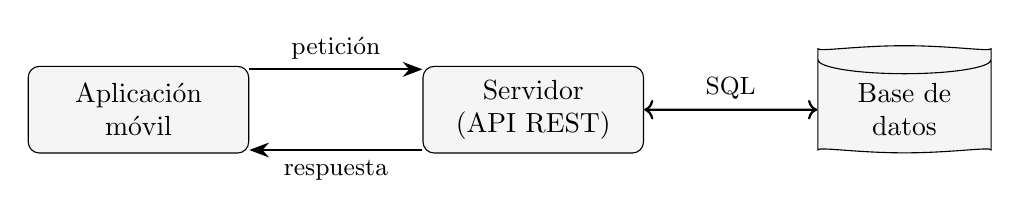
\begin{tikzpicture}[node distance=2.2cm,
      caja/.style={draw, rounded corners, minimum width=2.8cm, minimum height=1.1cm,
                   align=center, fill=gray!8},
      flecha/.style={-{Stealth[length=2.5mm]}, thick}]
    \node[caja] (cli) {Aplicación\\móvil};
    \node[caja, right=of cli] (srv) {Servidor\\(API REST)};
    \node[caja, right=of srv, shape=cylinder, shape border rotate=90, aspect=0.25,
          minimum width=2.2cm] (db) {Base de\\datos};
    \draw[flecha] (cli.20) -- node[above, font=\small] {petición} (srv.160);
    \draw[flecha] (srv.200) -- node[below, font=\small] {respuesta} (cli.340);
    \draw[flecha, <->] (srv) -- node[above, font=\small] {SQL} (db);
  \end{tikzpicture}
  \caption{Esquema de la arquitectura cliente-servidor del sistema.}
  \label{fig:cliente-servidor}
  \fuente{Elaboración propia a partir de~\cite{martin2022arquitectura}.}
\end{figure}

\subsection{Usabilidad y su medida}
\label{sec:usabilidad}

Cuando un trabajo usa una métrica, defínela con precisión. La \ac{SUS} es un
cuestionario de diez ítems que produce una puntuación entre 0 y
100 y que propuso Brooke~\cite{brooke1996sus}. Para cada participante, la
puntuación se calcula como
\begin{equation}
  \mathrm{SUS} = 2{,}5 \left( \sum_{i\ \text{impar}} (r_i - 1)
               + \sum_{i\ \text{par}} (5 - r_i) \right),
  \label{eq:sus}
\end{equation}
donde $r_i \in \{1,\dots,5\}$ es la respuesta al ítem $i$. La
Ecuación~\eqref{eq:sus} se usa en el Capítulo~\ref{cap:pruebas} para evaluar el
objetivo~\ref{obj:validacion}.

\section{Soluciones existentes}
\label{sec:soluciones}

En un \ac{TFG} de aplicación, este apartado es el estudio de mercado; en un
trabajo de investigación, la revisión de trabajos relacionados. En ambos casos
se analizan las alternativas con los mismos criterios y se resumen en una tabla.
En este ejemplo se han revisado tres aplicaciones (A, B y C), elegidas por ser
las más descargadas de su categoría en noviembre de
2026~\cite{informe_movil2025}, y un \ac{TFG} previo de la \ac{EPS} que abordó un
problema parecido con tecnologías web~\cite{ferrer2025tfg}.

% GUÍA: datos volátiles (descargas, valoraciones de tienda) siempre con fecha
% de consulta. Cada alternativa con su logo o captura si es una app.

La Tabla~\ref{tab:comparativa} compara las alternativas con los cuatro criterios
que se derivan de la motivación. Ninguna de las soluciones analizadas combina la
ocupación en tiempo real con la reserva desde el móvil, que es precisamente el
hueco que pretende cubrir \emph{SalaLibre}.

\begin{table}[htbp]
  \centering
  \caption{Comparativa de las soluciones existentes.}
  \label{tab:comparativa}
  \begin{tabularx}{\textwidth}{@{}lCCCC@{}}
    \toprule
    \textbf{Solución} & \textbf{Ocupación en tiempo real} & \textbf{Reserva móvil}
      & \textbf{Avisos} & \textbf{Código abierto} \\
    \midrule
    Aplicación A~\cite{ejemplo_appA} & $\times$ & \checkmark & \checkmark & $\times$ \\
    Aplicación B~\cite{ejemplo_appB} &\checkmark & $\times$ & $\times$ & $\times$ \\
    Aplicación C~\cite{garcia2024movil} & $\times$ & \checkmark & $\times$ & \checkmark \\
    \midrule
    \emph{SalaLibre} (este trabajo) & \checkmark & \checkmark & \checkmark & \checkmark \\
    \bottomrule
  \end{tabularx}
  \fuente{Elaboración propia a partir de las fuentes citadas (consulta: noviembre de 2026).}
\end{table}

\section{Conclusiones del capítulo}
\label{sec:conclusiones-estado}

Cierra el capítulo con dos o tres frases: qué se ha aprendido y qué decisión
se toma a partir de ello. En este caso, la falta de soluciones que integren
ocupación y reserva justifica el desarrollo de una aplicación propia, cuyos
requisitos se derivan de los criterios de la Tabla~\ref{tab:comparativa}.

% =====================================================================
%  CAPÍTULO 3 · METODOLOGÍA, PLANIFICACIÓN Y VIABILIDAD
%  Función: explicar CÓMO se ha trabajado y justificarlo.
%  Reglas clave:
%   - Justifica la metodología (por qué esta) y que su nombre corresponda al
%     proceso real («iterativa» solo si de verdad hubo iteraciones).
%   - Un ÚNICO plan: mismo número de fases y nombres en texto y Gantt.
%   - El plan llega hasta el depósito y la defensa, y se redacta en PASADO
%     en la memoria final («se desarrolló», no «se desarrollará»).
%   - Explica las desviaciones: lo planificado que no se hizo se declara.
%   - El stack se presenta UNA sola vez (aquí), con versión exacta y cita.
%   - El Portafoli evalúa la viabilidad económica y legal y la sostenibilidad.
% =====================================================================
\chapter{Metodología, planificación y viabilidad}
\label{cap:metodologia}

Este capítulo describe la metodología seguida, la planificación temporal real
del proyecto, las herramientas utilizadas y el análisis de su viabilidad.

\section{Metodología de desarrollo}
\label{sec:metodologia}

Se ha seguido un desarrollo iterativo e incremental en tres incrementos, cada
uno con análisis, implementación y pruebas propios. Se eligió este enfoque
porque los requisitos de tiempo real dependían de la validación del primer
incremento, y una planificación en cascada habría retrasado ese riesgo hasta el
final del proyecto~\cite{martin2022arquitectura}. Al final de cada incremento se
revisó el avance con la dirección del trabajo.

\section{Planificación temporal}
\label{sec:planificacion}

El proyecto se organizó en tres fases, que se muestran en la
Figura~\ref{fig:cronograma}. La fase de análisis (F1) se desarrolló entre
octubre y diciembre; la de diseño e implementación (F2), entre diciembre y
mayo, y la de validación y cierre (F3), entre mayo y julio, hasta el depósito y
la defensa. Los hitos en rojo corresponden a las entregas que evalúa el
Portafoli de la \ac{EPS}.

\begin{figure}[htbp]
  \centering
  % =====================================================================
%  CRONOGRAMA (diagrama de Gantt) · fuente ÚNICA de la planificación
%  Se usa en la memoria (Cap. 3) y en los informes inicial y de seguimiento:
%  así el plan es el mismo en todos los documentos.
%  - Una columna = una quincena (granularidad uniforme; no la mezcles).
%  - El plan llega SIEMPRE hasta el depósito y la defensa reales.
%  - progress=NN (opcional) marca el avance de una tarea en el seguimiento.
%  - Ajusta los meses y las fechas al calendario oficial del curso.
% =====================================================================
\begin{ganttchart}[
    x unit=0.45cm, y unit chart=0.52cm, y unit title=0.55cm,
    vgrid={*1{draw=black!10}}, hgrid,
    title label font=\scriptsize\bfseries, title height=1,
    bar label font=\footnotesize, group label font=\footnotesize\bfseries,
    milestone label font=\footnotesize\itshape,
    bar/.append style={fill=RoyalBlue!55, draw=RoyalBlue!80!black},
    group/.append style={fill=black!70},
    milestone/.append style={fill=BrickRed, draw=BrickRed},
    progress label text={}, bar incomplete/.append style={fill=RoyalBlue!15},
    bar height=0.55, group height=0.3, milestone height=0.55,
  ]{1}{20}
  \gantttitle{Oct}{2} \gantttitle{Nov}{2} \gantttitle{Dic}{2} \gantttitle{Ene}{2}
  \gantttitle{Feb}{2} \gantttitle{Mar}{2} \gantttitle{Abr}{2} \gantttitle{May}{2}
  \gantttitle{Jun}{2} \gantttitle{Jul}{2} \\
  \ganttgroup{F1. Análisis}{1}{6} \\
  \ganttbar{Propuesta y estado del arte}{1}{4} \\
  \ganttbar{Requisitos}{4}{6} \\
  \ganttgroup{F2. Diseño e implementación}{6}{15} \\
  \ganttbar{Diseño de la arquitectura}{6}{7} \\
  \ganttbar{Incremento 1: reservas}{8}{10} \\
  \ganttbar{Incremento 2: tiempo real}{11}{13} \\
  \ganttbar{Incremento 3: notificaciones}{14}{15} \\
  \ganttgroup{F3. Validación y cierre}{14}{20} \\
  \ganttbar{Pruebas y validación}{14}{17} \\
  \ganttbar{Redacción de la memoria}{3}{18} \\
  \ganttgroup{Hitos de evaluación}{3}{20} \\
  \ganttmilestone{Informe inicial (sem. 4-6)}{3} \\
  \ganttmilestone{Informe de seguimiento (sem. 10-12)}{6} \\
  \ganttmilestone{Documento final ($\geq$3 sem. antes)}{17} \\
  \ganttmilestone{Depósito ($\geq$5 días hábiles antes)}{19} \\
  \ganttmilestone{Defensa}{20}
\end{ganttchart}

  \caption{Planificación temporal del proyecto (por quincenas).}
  \label{fig:cronograma}
  \fuente{Elaboración propia.}
\end{figure}

\subsection{Desviaciones respecto al plan inicial}
\label{sec:desviaciones}

Compara lo planificado con lo realizado. Por ejemplo: el incremento 2 se
retrasó dos semanas porque la librería de notificaciones elegida no admitía el
modo sin conexión; se sustituyó por otra y se recortó el incremento 3. Si una
tarea planificada no se llegó a hacer (por ejemplo, una prueba con usuarios),
dilo aquí y en el capítulo de pruebas.

\section{Herramientas y tecnologías}
\label{sec:herramientas}

La Tabla~\ref{tab:herramientas} recoge las herramientas utilizadas, con su
versión exacta y el motivo de su elección. El resto de la memoria se refiere a
ellas sin volver a describirlas.

\begin{table}[htbp]
  \centering
  \caption{Herramientas y tecnologías utilizadas.}
  \label{tab:herramientas}
  \small
  \begin{tabularx}{\textwidth}{@{}lllL@{}}
    \toprule
    \textbf{Capa} & \textbf{Herramienta} & \textbf{Versión} & \textbf{Motivo de la elección} \\
    \midrule
    Cliente        & Kotlin~\cite{doc_kotlin}          & 2.0  & Lenguaje recomendado para Android \\
    Servidor       & Python~\cite{doc_python}          & 3.12 & Experiencia previa y ecosistema de pruebas \\
    API            & FastAPI~\cite{doc_fastapi}        & 0.115 & Documentación automática de la \ac{API} \\
    Datos          & PostgreSQL~\cite{doc_postgresql}  & 16   & Transacciones para evitar reservas dobles \\
    Despliegue     & Docker~\cite{doc_docker}          & 27   & Despliegue reproducible con un solo comando \\
    \bottomrule
  \end{tabularx}
  \fuente{Elaboración propia.}
\end{table}

% GUÍA: la versión debe ser la que REALMENTE usaste (mírala en tu proyecto).
% Justifica por adecuación al problema, no por popularidad
% («lo usa la empresa X» no es un motivo técnico).

\section{Viabilidad económica}
\label{sec:viabilidad-economica}

La Tabla~\ref{tab:presupuesto} estima el coste del proyecto. El coste de
personal se calcula con las horas reales de dedicación (un \ac{TFG} de 15 ECTS
supone unas 375 horas) y un coste por hora de referencia; el equipo se imputa
por amortización durante los meses de uso.

\begin{table}[htbp]
  \centering
  \caption{Presupuesto estimado del proyecto (datos de ejemplo).}
  \label{tab:presupuesto}
  \begin{tabular}{@{}lrrr@{}}
    \toprule
    \textbf{Concepto} & \textbf{Cantidad} & \textbf{Coste/ud. (€)} & \textbf{Total (€)} \\
    \midrule
    Horas de desarrollo                    & 375 h    & 20          & \num{7500} \\
    Portátil (amortización 9/48 meses)     & 1        & \num{1200}  & 225 \\
    Móvil de pruebas (amortización 9/36)   & 1        & 300         & 75 \\
    Servidor en la nube                    & 6 meses  & 10          & 60 \\
    Licencias de software                  & ---      & ---         & 0 \\
    \midrule
    \textbf{Total}                         &          &             & \textbf{\num{7860}} \\
    \bottomrule
  \end{tabular}
  \fuente{Elaboración propia.}
\end{table}

\section{Viabilidad legal}
\label{sec:viabilidad-legal}

Indica qué normativa afecta al proyecto y cómo se cumple. Si se tratan datos
personales, aplica el \ac{RGPD}~\cite{rgpd2016} y la ley orgánica española de
protección de datos~\cite{lopdgdd2018}: qué datos se guardan, con qué base
legal, durante cuánto tiempo y cómo se protegen. Revisa también las licencias de
las librerías que usas (y la que eliges para tu código) y, en una aplicación,
las pautas de accesibilidad~\cite{wcag22}.

\section{Sostenibilidad e impacto social}
\label{sec:sostenibilidad}

Valora brevemente el impacto social, económico y ambiental de la solución: a
quién beneficia, qué recursos consume (por ejemplo, energía del servidor o
batería del móvil) y con qué Objetivos de Desarrollo Sostenible se relaciona.

% =====================================================================
%  CAPÍTULO 4 · ANÁLISIS Y DISEÑO
%  Función: definir QUÉ debe hacer el sistema (requisitos verificables) y
%  CÓMO se ha decidido construirlo (arquitectura y decisiones justificadas).
%  Reglas clave:
%   - Requisitos con ID (RF-01, RNF-01), atómicos y verificables. Di de
%     dónde salen (estado del arte, entrevistas, normativa...).
%   - Lo que no has medido no se afirma como cumplido («cumple WCAG AA»
%     solo si lo has comprobado y lo muestras).
%   - Cada diagrama se explica en el texto componente a componente.
%   - Trabajos con datos/ML: añade aquí (o en el Cap. 5) una ficha por
%     dataset: estructura, nº de muestras y particiones, tipo de dato con
%     un ejemplo visual, referencia y protocolo de evaluación.
% =====================================================================
\chapter{Análisis y diseño}
\label{cap:diseno}

Este capítulo especifica los requisitos de \emph{SalaLibre} y describe la
arquitectura y las decisiones de diseño que se tomaron para cumplirlos.

\section{Requisitos}
\label{sec:requisitos}

Los requisitos se obtuvieron de la comparativa del
Capítulo~\ref{cap:estado} y de una entrevista con el personal de la biblioteca.
Cada requisito tiene un identificador que se usa en las pruebas del
Capítulo~\ref{cap:pruebas}. La Tabla~\ref{tab:rf} recoge los requisitos
funcionales y la Tabla~\ref{tab:rnf}, los no funcionales.

\begin{table}[htbp]
  \centering
  \caption{Requisitos funcionales (extracto).}
  \label{tab:rf}
  \small
  \begin{tabularx}{\textwidth}{@{}lLl@{}}
    \toprule
    \textbf{ID} & \textbf{Descripción} & \textbf{Objetivo} \\
    \midrule
    RF-01 & El usuario puede consultar las salas libres en este momento. & \ref{obj:app} \\
    RF-02 & El usuario puede reservar una sala libre en dos pasos como máximo. & \ref{obj:app} \\
    RF-03 & El usuario recibe una notificación 10 minutos antes de su reserva. & \ref{obj:app} \\
    RF-04 & El sistema impide dos reservas solapadas de la misma sala. & \ref{obj:app} \\
    \bottomrule
  \end{tabularx}
  \fuente{Elaboración propia.}
\end{table}

\begin{table}[htbp]
  \centering
  \caption{Requisitos no funcionales (extracto).}
  \label{tab:rnf}
  \small
  \begin{tabularx}{\textwidth}{@{}lLl@{}}
    \toprule
    \textbf{ID} & \textbf{Descripción y criterio de aceptación} & \textbf{Objetivo} \\
    \midrule
    RNF-01 & Rendimiento: latencia media $<$ \qty{100}{ms} con 200 usuarios concurrentes. & \ref{obj:rendimiento} \\
    RNF-02 & Usabilidad: puntuación \ac{SUS} media $\geq 70$ con al menos 8 usuarios. & \ref{obj:validacion} \\
    RNF-03 & Seguridad: las contraseñas se almacenan con una función de \emph{hash} con sal. & \ref{obj:app} \\
    \bottomrule
  \end{tabularx}
  \fuente{Elaboración propia.}
\end{table}

% GUÍA: «El sistema será escalable» NO es verificable. Da un criterio medible
% o márcalo explícitamente como objetivo de diseño no medido.

\section{Arquitectura del sistema}
\label{sec:arquitectura}

La Figura~\ref{fig:arquitectura} muestra la arquitectura en tres capas. La capa
de presentación (arriba) es la aplicación Android, que solo se comunica con el
servidor mediante la \ac{API}. La capa de lógica (centro) valida las reservas y
envía las notificaciones. La capa de datos (abajo) guarda salas, usuarios y
reservas. Se eligió separar la lógica en el servidor para que la regla RF-04
(sin reservas solapadas) se compruebe en un único punto, dentro de una
transacción de la base de datos.

\begin{figure}[htbp]
  \centering
  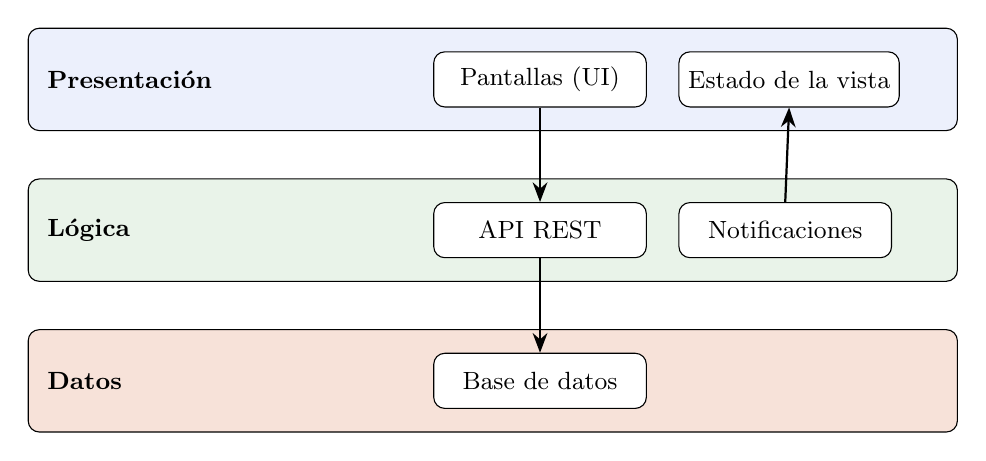
\begin{tikzpicture}[
      capa/.style={draw, rounded corners, minimum width=11.8cm, minimum height=1.3cm,
                   align=center, fill=#1},
      comp/.style={draw, rounded corners, fill=white, minimum width=2.7cm,
                   minimum height=0.7cm, font=\small},
      flecha/.style={-{Stealth[length=2.5mm]}, thick}]
    \node[capa=RoyalBlue!10] (pres) {};
    \node[anchor=west, font=\small\bfseries] at (pres.west) {\ Presentación};
    \node[comp] at ([xshift=0.6cm]pres.center) (ui) {Pantallas (UI)};
    \node[comp, right=0.4cm of ui] (vm) {Estado de la vista};
    \node[capa=ForestGreen!10, below=0.6cm of pres] (log) {};
    \node[anchor=west, font=\small\bfseries] at (log.west) {\ Lógica};
    \node[comp] at ([xshift=0.6cm]log.center) (api) {API REST};
    \node[comp, right=0.4cm of api] (not) {Notificaciones};
    \node[capa=BrickRed!10, below=0.6cm of log] (dat) {};
    \node[anchor=west, font=\small\bfseries] at (dat.west) {\ Datos};
    \node[comp] at ([xshift=0.6cm]dat.center) (db) {Base de datos};
    \draw[flecha] (ui) -- (api);
    \draw[flecha] (api) -- (db);
    \draw[flecha] (not.north) -- (vm.south);
  \end{tikzpicture}
  \caption{Arquitectura en capas de \emph{SalaLibre}.}
  \label{fig:arquitectura}
  \fuente{Elaboración propia.}
\end{figure}

\section{Diseño de la interfaz}
\label{sec:diseno-interfaz}

En una aplicación, muestra los prototipos (\emph{wireframes}) y el mapa de
navegación, y relaciónalos con los requisitos. La
Figura~\ref{fig:navegacion} resume la navegación: desde la pantalla de inicio se
llega a la reserva en dos pasos, como exige RF-02.

\begin{figure}[htbp]
  \centering
  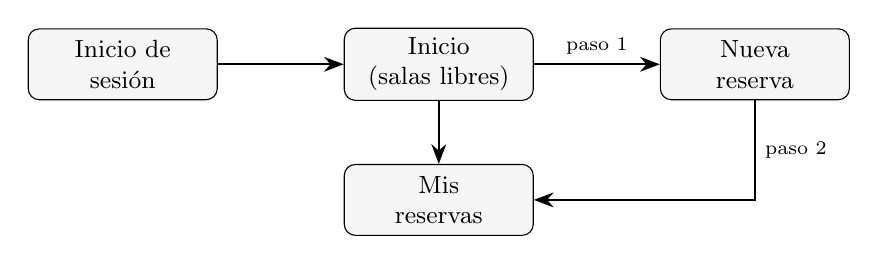
\begin{tikzpicture}[node distance=1.6cm,
      pant/.style={draw, rounded corners, fill=gray!8, minimum width=2.4cm,
                   minimum height=0.9cm, align=center, font=\small},
      flecha/.style={-{Stealth[length=2.5mm]}, thick}]
    \node[pant] (login) {Inicio de\\sesión};
    \node[pant, right=of login] (inicio) {Inicio\\(salas libres)};
    \node[pant, right=of inicio] (reserva) {Nueva\\reserva};
    \node[pant, below=0.8cm of inicio] (mis) {Mis\\reservas};
    \draw[flecha] (login) -- (inicio);
    \draw[flecha] (inicio) -- node[above, font=\scriptsize] {paso 1} (reserva);
    \draw[flecha] (reserva.south) |- node[pos=0.25, right, font=\scriptsize] {paso 2} (mis.east);
    \draw[flecha] (inicio) -- (mis);
  \end{tikzpicture}
  \caption{Mapa de navegación de la aplicación.}
  \label{fig:navegacion}
  \fuente{Elaboración propia.}
\end{figure}

% =====================================================================
%  CAPÍTULO 5 · IMPLEMENTACIÓN
%  Función: contar cómo se ha construido la solución y conectar cada parte
%  con los requisitos. Que se vea el trabajo real.
%  Reglas clave:
%   - Organiza por componentes, no por orden cronológico.
%   - Estructura del código y cómo se conectan los componentes.
%   - Fragmentos de código SOLO si aportan (10-25 líneas) y siempre
%     explicados; el código completo va en el repositorio (Apéndice A).
%   - En una app: capturas REALES de la aplicación, agrupadas (2-3 por
%     figura), y legibles.
%   - Explica errores, seguridad y privacidad donde apliquen.
%   - Definiciones técnicas exactas (p. ej. qué se cifra y con qué).
% =====================================================================
\chapter{Implementación}
\label{cap:implementacion}

Este capítulo describe cómo se han implementado los componentes de la
arquitectura presentada en la Sección~\ref{sec:arquitectura}.

\section{Estructura del código}
\label{sec:estructura-codigo}

El código se organiza en dos módulos dentro del mismo repositorio
(Apéndice~\ref{ap:repositorio}): \texttt{app/}, con la aplicación Android, y
\texttt{servidor/}, con la \ac{API} y el acceso a datos. El
Listado~\ref{lst:estructura} muestra las carpetas principales del servidor.

\begin{lstlisting}[float, language={}, numbers=none, caption={Estructura de carpetas del servidor.},
                   label={lst:estructura}]
servidor/
|-- api/          rutas de la API (salas, reservas, usuarios)
|-- dominio/      reglas de negocio (p. ej. solapamiento de reservas)
|-- datos/        acceso a la base de datos
`-- pruebas/      pruebas unitarias y de integración
\end{lstlisting}

\section{Gestión de reservas}
\label{sec:gestion-reservas}

La regla que impide reservas solapadas (RF-04) es la parte más delicada del
sistema, porque dos usuarios pueden intentar reservar la misma sala a la vez. El
Listado~\ref{lst:reserva} muestra cómo se resuelve: la comprobación y la
inserción se ejecutan dentro de una misma transacción (línea 4), de modo que la
segunda petición ve la reserva de la primera y recibe un error 409 (línea 10) en
lugar de crear un duplicado.

% [float]: el listado se coloca entero donde quepa, sin partirse entre páginas.
\begin{lstlisting}[float, language=Python, caption={Creación de una reserva sin solapamientos.},
                   label={lst:reserva}]
@router.post("/reservas", status_code=201)
def crear_reserva(datos: ReservaIn, db: Session = Depends(get_db)):
    """Crea una reserva si la sala está libre en esa franja (RF-04)."""
    with db.begin():                       # una única transacción
        solapada = db.query(Reserva).filter(
            Reserva.sala_id == datos.sala_id,
            Reserva.inicio < datos.fin, Reserva.fin > datos.inicio,
        ).with_for_update().first()
        if solapada:
            raise HTTPException(409, "La sala ya está reservada")
        reserva = Reserva(**datos.dict())
        db.add(reserva)
    return reserva
\end{lstlisting}

\section{Aplicación móvil}
\label{sec:app}

La Figura~\ref{fig:capturas} muestra dos pantallas reales de la aplicación. En
la pantalla de inicio (Figura~\ref{fig:captura-inicio}) el usuario ve qué salas
están libres en ese momento (RF-01); al pulsar una sala libre pasa directamente
al formulario de reserva (Figura~\ref{fig:captura-reserva}), que solo pide la
franja y el número de asistentes, de modo que la reserva se completa en dos
pasos (RF-02).

\begin{figure}[htbp]
  \centering
  \begin{subfigure}[b]{0.32\textwidth}
    \centering
    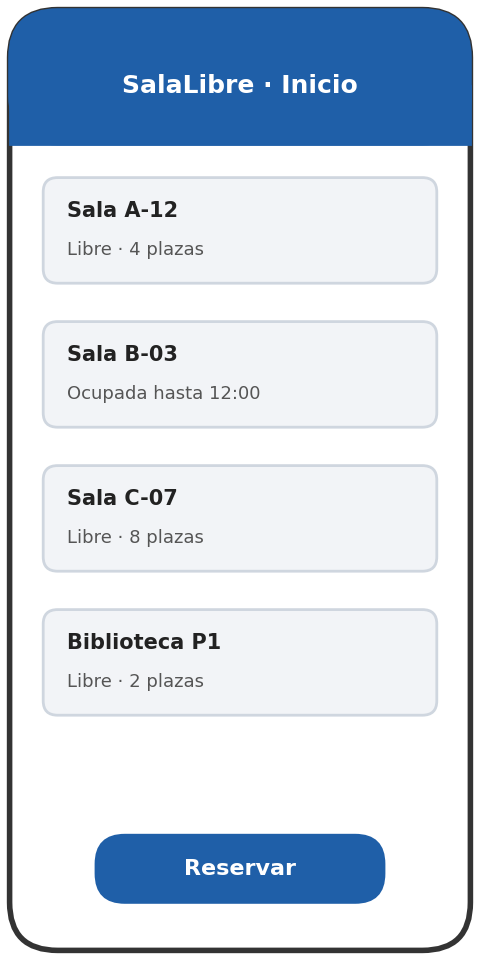
\includegraphics[width=\linewidth]{captura_inicio}
    \caption{Pantalla de inicio.}
    \label{fig:captura-inicio}
  \end{subfigure}\hspace{1.5cm}%
  \begin{subfigure}[b]{0.32\textwidth}
    \centering
    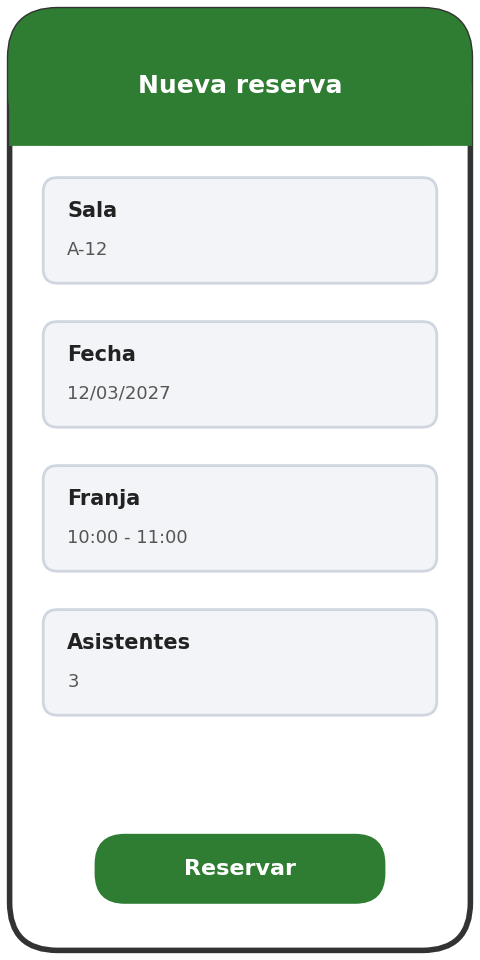
\includegraphics[width=\linewidth]{captura_reserva}
    \caption{Formulario de reserva.}
    \label{fig:captura-reserva}
  \end{subfigure}
  \caption{Pantallas principales de la aplicación.}
  \label{fig:capturas}
  \fuente{Elaboración propia (capturas de la aplicación).}
\end{figure}

% GUÍA: para una app, graba además un vídeo demo (YouTube no listado) y
% enlázalo con URL y código QR (Apéndice A). La memoria debe entenderse
% igualmente sin el vídeo.

\section{Seguridad y gestión de errores}
\label{sec:seguridad}

Explica las decisiones de seguridad con precisión técnica. Por ejemplo: las
contraseñas se guardan con una función de \emph{hash} con sal (RNF-03) y nunca
viajan en claro; las sesiones se gestionan con un \emph{token} firmado por el
servidor. Describe también qué ve el usuario cuando falla la red o una
petición, y cómo se registran los errores en el servidor.

% =====================================================================
%  CAPÍTULO 6 · PRUEBAS Y RESULTADOS
%  Función: demostrar CON EVIDENCIA que se cumplen requisitos y objetivos.
%  Reglas clave:
%   - Casos de prueba con entrada/pasos -> resultado esperado -> obtenido.
%     «Se ha probado manualmente» no es evidencia.
%   - NUNCA presentes como hecho algo propuesto o futuro: si una prueba no
%     se pudo hacer, dilo explícitamente.
%   - Cifras coherentes entre texto, tablas y resumen. Con usuarios:
%     N, perfil, instrumento y valores absolutos («6 de 8», no solo «75 %»).
%   - Cada gráfica se interpreta: qué se ve, qué significa, qué se decide.
%   - Las hipótesis no son hechos («indicios de», no «se confirma»).
% =====================================================================
\chapter{Pruebas y resultados}
\label{cap:pruebas}

Este capítulo presenta la estrategia de pruebas, los resultados obtenidos y su
relación con los requisitos y los objetivos del trabajo.

\section{Estrategia de pruebas}
\label{sec:estrategia}

Se han realizado tres tipos de pruebas: pruebas funcionales de cada requisito,
pruebas de carga para el requisito de rendimiento (RNF-01) y una prueba de
usabilidad con usuarios (RNF-02). Las pruebas funcionales y de carga se
ejecutaron sobre la versión etiquetada \texttt{\tfgversion} del repositorio
(Apéndice~\ref{ap:repositorio}).

\section{Pruebas funcionales}
\label{sec:pruebas-funcionales}

La Tabla~\ref{tab:casos} recoge los casos de prueba de los requisitos
funcionales. Los cuatro casos se superaron; el caso PR-04, que simula dos
reservas simultáneas de la misma sala, confirma que la transacción del
Listado~\ref{lst:reserva} evita el solapamiento.

\begin{table}[htbp]
  \centering
  \caption{Casos de prueba funcionales.}
  \label{tab:casos}
  \small
  \begin{tabularx}{\textwidth}{@{}llLLl@{}}
    \toprule
    \textbf{ID} & \textbf{Req.} & \textbf{Pasos / entrada} & \textbf{Resultado esperado} & \textbf{Estado} \\
    \midrule
    PR-01 & RF-01 & Abrir la app con dos salas libres & Se listan las dos salas & Superada \\
    PR-02 & RF-02 & Reservar la sala A-12 desde el inicio & Reserva creada en 2 pasos & Superada \\
    PR-03 & RF-03 & Reserva a 11 min vista & Aviso a los 10 min & Superada \\
    PR-04 & RF-04 & Dos peticiones simultáneas a la misma franja & Una creada, otra con error 409 & Superada \\
    \bottomrule
  \end{tabularx}
  \fuente{Elaboración propia.}
\end{table}

\section{Pruebas de rendimiento}
\label{sec:rendimiento}

Se midió la latencia media de la \ac{API} con 10 a 400 usuarios concurrentes
simulados, repitiendo cada medida cinco veces. La
Figura~\ref{fig:latencia} compara la versión inicial con la versión que añade
una caché de consultas. Sin caché, la latencia supera el umbral de
\qty{100}{ms} a partir de unos 200 usuarios; con caché, se mantiene por debajo
del umbral en todo el rango medido, con \qty{92}{ms} para 400 usuarios. Por
tanto, RNF-01 se cumple con margen y el objetivo~\ref{obj:rendimiento} se
alcanza.

\begin{figure}[htbp]
  \centering
  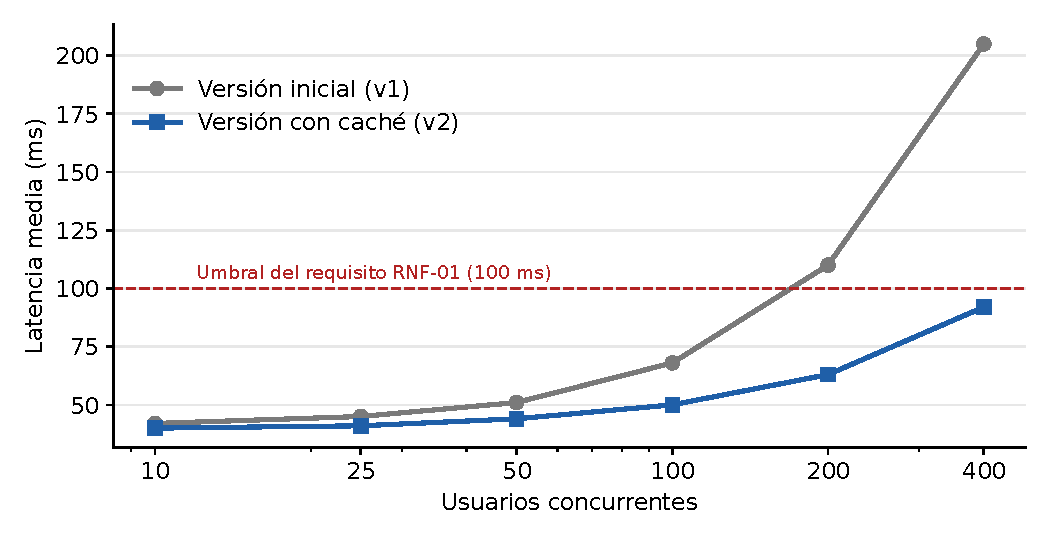
\includegraphics[width=\textwidth]{resultados_latencia}
  \caption{Latencia media de la API según el número de usuarios concurrentes.}
  \label{fig:latencia}
  \fuente{Elaboración propia (datos de ejemplo, ficticios).}
\end{figure}

% GUÍA: las gráficas de datos van a ANCHO COMPLETO, con ejes etiquetados y
% unidades. Expórtalas en vectorial (PDF) desde tu script y guarda el script
% en el repositorio para poder regenerarlas.

\section{Prueba de usabilidad}
\label{sec:usabilidad-resultados}

Ocho estudiantes de grado, sin relación con el proyecto, realizaron tres tareas
de reserva y respondieron después el cuestionario \ac{SUS}
(Ecuación~\ref{eq:sus}). La puntuación media fue de 81 (desviación típica 7),
por encima del umbral de 70 fijado en RNF-02. Siete de los ocho participantes
(88\,\%) completaron todas las tareas sin ayuda; el único error repetido fue no
encontrar el botón de cancelar una reserva, que se movió en el incremento 3.

% GUÍA: si la prueba con usuarios NO se pudo hacer, escríbelo así:
% «La prueba de usabilidad prevista en la planificación no se ha podido
% realizar; se propone como trabajo futuro (Sección 7.3).»

\section{Trazabilidad y resumen de resultados}
\label{sec:trazabilidad}

La Tabla~\ref{tab:trazabilidad} relaciona cada objetivo con los requisitos que
lo concretan y con las pruebas que lo validan, y resume el resultado obtenido.

\begin{table}[htbp]
  \centering
  \caption{Trazabilidad entre objetivos, requisitos y pruebas.}
  \label{tab:trazabilidad}
  \small
  \begin{tabularx}{\textwidth}{@{}llLL@{}}
    \toprule
    \textbf{Objetivo} & \textbf{Requisitos} & \textbf{Evidencia} & \textbf{Resultado} \\
    \midrule
    \ref{obj:estado}      & ---           & Tabla~\ref{tab:comparativa}  & Comparativa de 3 soluciones \\
    \ref{obj:app}         & RF-01 a RF-04 & PR-01 a PR-04 (Tabla~\ref{tab:casos}) & 4/4 pruebas superadas \\
    \ref{obj:rendimiento} & RNF-01        & Figura~\ref{fig:latencia}    & \qty{92}{ms} con 400 usuarios \\
    \ref{obj:validacion}  & RNF-02        & Sección~\ref{sec:usabilidad-resultados} & SUS = 81 ($n = 8$) \\
    \bottomrule
  \end{tabularx}
  \fuente{Elaboración propia.}
\end{table}

\section{Discusión y limitaciones}
\label{sec:discusion}

Interpreta los resultados con espíritu crítico: qué significan, qué no
demuestran y qué podría haber influido. En este ejemplo, las pruebas de carga
se hicieron en un único servidor y con usuarios simulados, y la prueba de
usabilidad tiene una muestra pequeña ($n = 8$), por lo que los resultados son
indicativos y no generalizables a todo el campus.

% =====================================================================
%  CAPÍTULO 7 · CONCLUSIONES Y TRABAJO FUTURO
%  Función: cerrar el círculo. Cada objetivo de la Sección 1.3 se retoma
%  UNO A UNO: cumplido / parcialmente / no cumplido, con su evidencia.
%  Reglas clave:
%   - No introduzcas aquí resultados nuevos que no estén en el Cap. 6.
%   - Limitaciones (lo que no salió) separadas del trabajo futuro.
%   - Trabajo futuro: ~1 página, concreto y ligado a limitaciones reales.
% =====================================================================
\chapter{Conclusiones y trabajo futuro}
\label{cap:conclusiones}

Este capítulo valora el grado de cumplimiento de los objetivos, resume las
aportaciones y las limitaciones del trabajo y propone líneas de continuación.

\section{Cumplimiento de los objetivos}
\label{sec:cumplimiento}

La Tabla~\ref{tab:cumplimiento} resume el estado final de cada objetivo
específico planteado en la Sección~\ref{sec:objetivos}.

\begin{table}[htbp]
  \centering
  \caption{Grado de cumplimiento de los objetivos.}
  \label{tab:cumplimiento}
  \small
  \begin{tabularx}{\textwidth}{@{}lLlL@{}}
    \toprule
    \textbf{Obj.} & \textbf{Descripción} & \textbf{Estado} & \textbf{Evidencia} \\
    \midrule
    \ref{obj:estado}      & Comparativa de soluciones   & Cumplido & Sección~\ref{sec:soluciones} \\
    \ref{obj:app}         & Aplicación Android funcional & Cumplido & Tabla~\ref{tab:casos} \\
    \ref{obj:rendimiento} & Latencia $<$ \qty{100}{ms}   & Cumplido & Figura~\ref{fig:latencia} \\
    \ref{obj:validacion}  & Validación con usuarios      & Parcial  & SUS = 81, pero $n = 8$ (Sección~\ref{sec:discusion}) \\
    \bottomrule
  \end{tabularx}
  \fuente{Elaboración propia.}
\end{table}

Desarrolla después cada objetivo en uno o dos párrafos. Por ejemplo: el
objetivo~\ref{obj:rendimiento} se ha cumplido, ya que con la caché la latencia
media se mantiene en \qty{92}{ms} con 400 usuarios, el doble de la carga exigida
por RNF-01. El objetivo~\ref{obj:validacion} se considera parcialmente cumplido:
la puntuación supera el umbral, pero la muestra es pequeña.

\section{Conclusiones}
\label{sec:conclusiones}

Resume qué aporta el trabajo y qué se ha aprendido, tanto en lo técnico como en
la gestión del proyecto. Las conclusiones se apoyan en los resultados del
Capítulo~\ref{cap:pruebas}; no repitas la introducción ni añadas afirmaciones
que no se hayan demostrado.

\section{Limitaciones}
\label{sec:limitaciones}

Enumera con honestidad lo que el trabajo no cubre o no ha podido validar y por
qué: por ejemplo, la ausencia de pruebas en varios servidores o la muestra
reducida de la prueba de usabilidad.

\section{Trabajo futuro}
\label{sec:futuro}

Propón tres o cuatro líneas concretas y priorizadas, cada una ligada a una
limitación. Por ejemplo: repetir la prueba de usabilidad con al menos treinta
usuarios de distintos grados; desplegar el servidor en dos nodos para medir la
escalabilidad horizontal, y publicar una versión para iOS.


% =====================================================================
%  BIBLIOGRAFÍA Y APÉNDICES
% =====================================================================
\printbibliography[heading=bibintoc]

\appendix
% =====================================================================
%  APÉNDICE A · REPOSITORIO Y VÍDEO DE DEMOSTRACIÓN
%  - Enlaza el repositorio con la versión exacta entregada (tag o commit).
%  - Apps: vídeo demo en YouTube (puede ser «no listado») con URL y QR.
%    Comprueba que el enlace funciona y que el QR se lee con el móvil.
%  - Todo apéndice debe citarse desde el cuerpo («ver Apéndice A»).
% =====================================================================
\chapter{Repositorio y vídeo de demostración}
\label{ap:repositorio}

El código fuente completo, los \emph{scripts} de las pruebas y los datos de las
figuras están disponibles en el repositorio del proyecto. La versión evaluada
en esta memoria corresponde a la etiqueta \texttt{\tfgversion}:

\begin{center}
  \url{\tfgrepo}
\end{center}

El vídeo de la Figura~\ref{fig:qr} muestra el funcionamiento de la aplicación
en un dispositivo real: consulta de salas libres, reserva y notificación.

\begin{figure}[htbp]
  \centering
  {\hypersetup{urlcolor=black}\qrcode[height=3.2cm]{\tfgvideo}}
  \caption{Código QR del vídeo de demostración.}
  \label{fig:qr}
  \fuente{\url{\tfgvideo}}
\end{figure}

% =====================================================================
%  APÉNDICE B · MANUAL DE INSTALACIÓN Y USO
%  Objetivo: que otra persona pueda ejecutar el proyecto. Lo ideal es un
%  único comando (p. ej. docker compose) y los requisitos previos exactos.
% =====================================================================
\chapter{Manual de instalación}
\label{ap:manual}

Este apéndice explica cómo poner en marcha el sistema descrito en el
Capítulo~\ref{cap:implementacion}. Solo se necesita Docker~\cite{doc_docker} y
una copia del repositorio (Apéndice~\ref{ap:repositorio}). El
Listado~\ref{lst:instalacion} muestra los comandos.

\begin{lstlisting}[float, language=bash, caption={Puesta en marcha del servidor.},
                   label={lst:instalacion}]
git clone https://github.com/usuario/repositorio.git
cd repositorio
docker compose up -d          # base de datos + API en http://localhost:8000
docker compose run --rm api pytest   # ejecuta todas las pruebas
\end{lstlisting}

La aplicación Android se instala desde el fichero \texttt{app-release.apk}
publicado en la sección de \emph{releases} del repositorio.


\end{document}
